\begin{spacing}{2}

With the constant growth of science and technology in our society, the world has witnessed an overall better life expectancy and reduced mortality rate: owing to improved living standards, better medical facilities and safer man-made environments. This ever-growing population has led to high demands of increased productivity of uniform quality end products for consumption. The industry has thus started shifting towards computer based automation and use of machinery to reduce manufacturing time and eliminate potential human error. These purpose specific machines, \textit{hard automation systems}, are a common practise in-spite of their inflexible and expensive nature. Thus, creating the need for reliable, flexible and low-cost robotic solutions.

The term \textit{Robot} was originally coined in \textit{1920} by Czech playwright Karol Capek in his play \textit{Rossum's Universal Robots}. Robot has been derived from Czech word \textit{robota} meaning \textbf{work}. This was used to portray robots as mechanical slaves which were developed to reduce human efforts by replacing humans where similar tasks were to be performed repeatedly.

In 1979, the \textbf{Robot Institute of America} (RIA) provided an official definition for a \textit{Robot} as follows:

\textit{"A robot is a reprogrammable, multifunctional manipulator designed to move material, parts, tools or specialized devices through variable programmed motions for the performance of a variety of tasks."}

Robots can be broadly categories into \textit{Fixed} or \textit{Mobile} robots based on mobility as depicted in Fig \ref{fig:classification}.

\subsubsection*{Fixed Robots}
The definition given above typically refers to a robotic manipulator which is commonly used in the manufacturing industry for the purpose of pick and place operations, welding, assembly and spraying. These robots are usually attached to an immobile base, thus classified as \textit{Fixed robots}. 
\begin{figure}
    \centering
    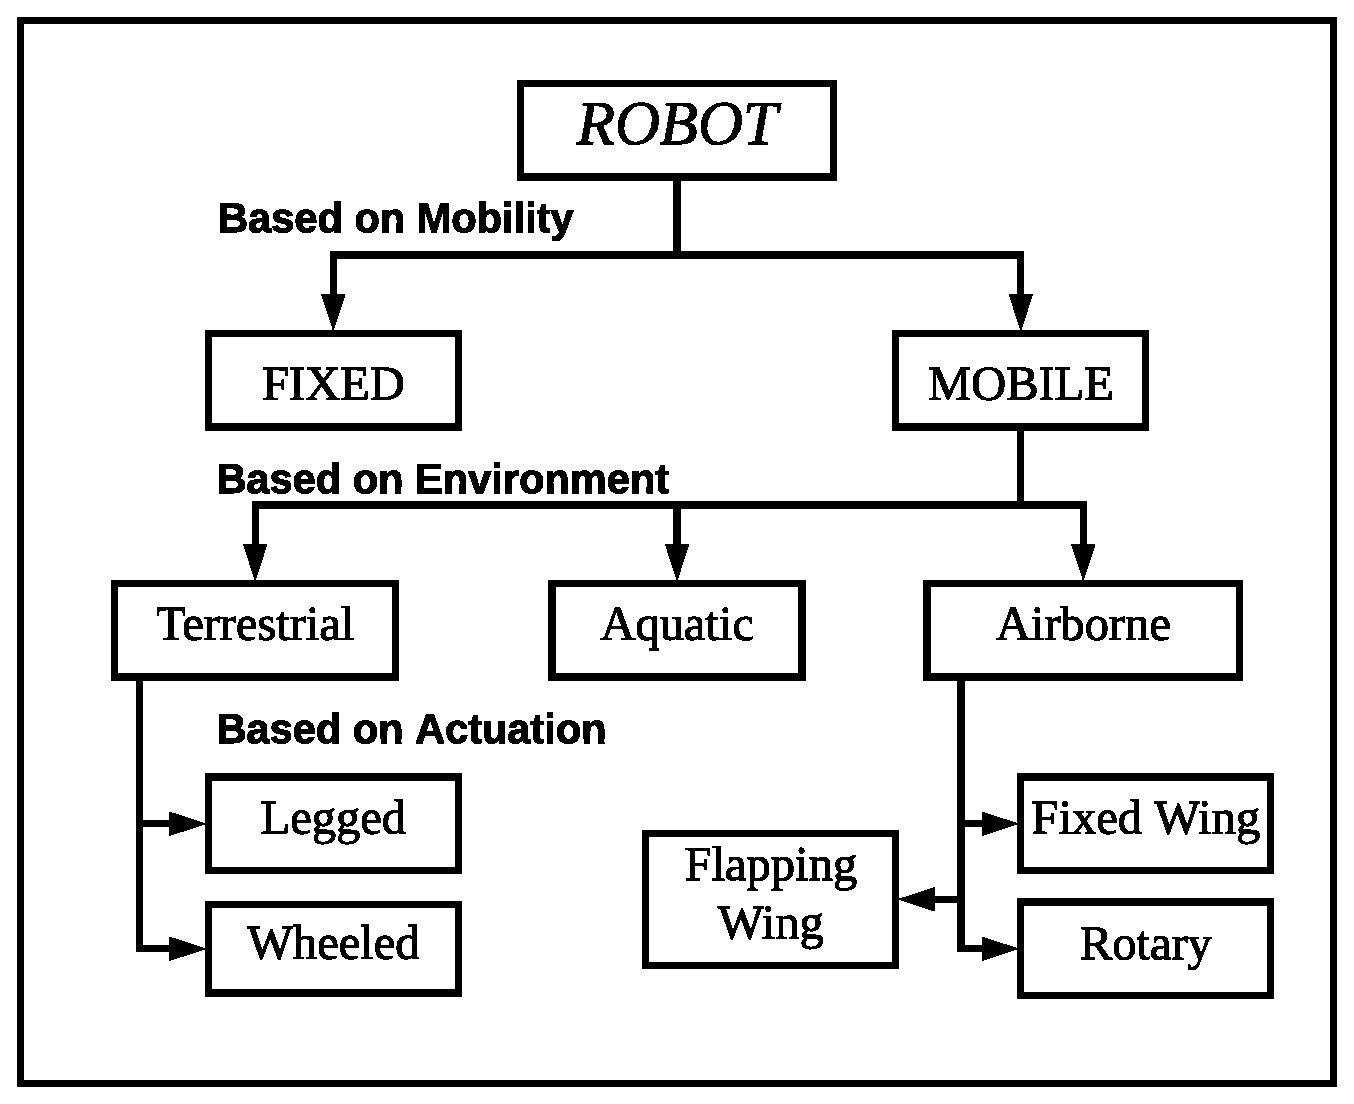
\includegraphics[width=0.8\linewidth]{image/robot_classification.eps}
    \caption{Robot Classification}
    \label{fig:classification}
\end{figure}

 Fixed robots, usually robotic manipulators, consists of a series of links and joints. These joints can be either \textbf{Prismatic} (linear) or \textbf{Revolute} (rotary). They are broadly divided into the following 4 categories based on their physical configuration as depicted in Fig \ref{fig:manipulator_config}:
\begin{enumerate}
    \item Cartesian Coordinate Robot
    \item Cylindrical Coordinate Robot
    \item Polar Coordinate Robot
    \item Articulated Arm Robot
\end{enumerate}

\begin{figure}[h]
 
\begin{subfigure}{0.5\textwidth}
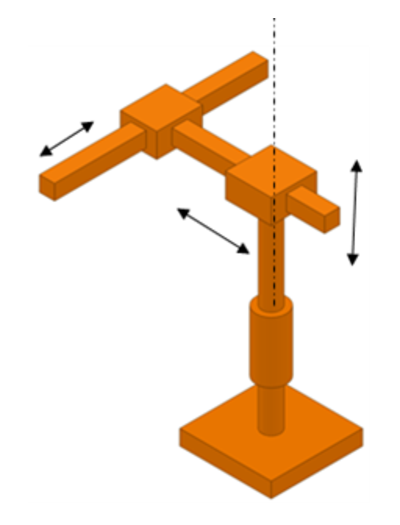
\includegraphics[width=0.9\linewidth, height=5cm]{image/cartesian.eps} 
\caption{Cartesian Coordinate Robot}
\end{subfigure}
\begin{subfigure}{0.5\textwidth}
\includegraphics[width=0.9\linewidth, height=5cm]{image/cylindrical.eps}
\caption{Cylindrical Coordinate Robot}
\end{subfigure}
 
 \begin{subfigure}{0.5\textwidth}
\includegraphics[width=0.9\linewidth, height=5cm]{image/polar.eps} 
\caption{Polar Coordinate Robot}
\end{subfigure}
\begin{subfigure}{0.5\textwidth}
\includegraphics[width=0.9\linewidth, height=5cm]{image/articulated.eps}
\caption{Articulated Arm Robot}
\end{subfigure}

\caption[Caption for LOF]{Physical Configurations of Fixed Robotic Manipulator\protect\footnotemark}
\label{fig:manipulator_config}
\end{figure}
\footnotetext{Courtesy of https://nptel.ac.in/courses/112103174/module7/lec5/3.html}
\subsubsection*{Mobile Robots}

Mobile robots are a class of robots which possess locomotion capabilities. While fixed robotics manipulators have witnessed large growth due to their massive use in the industries, mobile robotics is a relatively new field. The field of mobile robotics has been found to gain interest due to open-source projects and independent research work performed by academic researchers. These systems are being tested extensively for use in potential applications such as warehouse automation, surveillance, disaster relief and military applications.

Mobile robots are further classified on the basis of the environment in which they operate into three broad categories as depicted in Fig \ref{fig:classification} as follows:
\begin{enumerate}
    \item Terrestrial Robots
    \item Aquatic Robots
    \item Airborne / Aerial Robots
\end{enumerate}

\begin{figure}[h]
 
\begin{subfigure}{0.5\textwidth}
\includegraphics[width=0.45\linewidth, height=3cm]{image/quadraped.jpg} \includegraphics[width=0.45\linewidth, height=3cm]{image/rover.jpg}
\caption{Terrestrial Robot [Legged, Wheeled]}
\end{subfigure}
\begin{subfigure}{0.5\textwidth}
\includegraphics[width=0.45\linewidth, height=3cm, trim= 100 50 100 50,clip]{image/auv.jpg}
\includegraphics[width=0.45\linewidth, height=3cm, trim= 20 0 50 10,clip]{image/softfish.jpg}
\caption{Aquatic Robot}
\end{subfigure}
\begin{subfigure}{\textwidth}
\includegraphics[width=0.23\linewidth, height=3.5cm, trim= 100 10 20 20,clip]{image/quad.jpg} \includegraphics[width=0.23\linewidth, height=3.5cm, trim= 10 40 5 50,clip]{image/fixedwing.jpg}
\includegraphics[width=0.23\linewidth, height=3.5cm, trim= 5 30 5 40,clip]{image/helicopter.jpg} \includegraphics[width=0.23\linewidth, height=3.5cm, trim= 0 70 0 50,clip]{image/smartbird.jpg}
\caption{Aerial Robot [Multirotor, Plane, Helicopter, Flapping Wing]}
\end{subfigure}

\caption{Mobile Robotic Platforms}
\label{fig:mobile robot}
\end{figure}

Fig \ref{fig:mobile robot} shows some of the common mobile robots from different categories. There also exist some robotic system which can operate in more than one kind of environment, these systems however are out of the scope of this report. The usage of each of these robotic systems vary significantly based on the environment and user. The rest of the report emphasises majorly on the \textit{Aerial Robots}.

\section{Aerial Robots}

Aerial robots are a subclass of mobile robotic systems that possess the ability to aviate and navigate in aerial environment, or simply put, these are the robots which can fly. The ability to fly leads to an exponential rise in the applications at the cost of limitations like reduced endurance, higher cost, difficult operation and maintenance. Aerial robots are broadly classified into copters, planes and flapping wing vehicles based on the mechanism used to produce lift for the purpose of flying. Other classifications can be done based on autonomy, presence of pilot and passengers, payload capacity and gross take-off weight. We consider the use of unmanned vehicles only for this report.

An unmanned aerial vehicle (UAV), is an aircraft without a human pilot onboard. Also known as drones, UAVs form a crucial part of an unmanned aerial system (UAS); which includes a UAV, remote operator, ground control station and communication between these. The degree of autonomy of a UAV may range from remote-piloting to autonomous on-board control.

\subsubsection*{Plane}
An airplane (informally plane) is a fixed-wing aircraft, powered and propelled forward using the thrust generated from a engine or propeller. They rely on the relative motion of wings with respect to air to generate lift. Airplanes can have a large variety of sizes, shapes, and wing configurations (like high wing, low wing, biplanes, canards, blended wing bodies) which can be observed being used in RC hobby platforms. They are more efficient and thus used for lifting heavy payloads over large distances. The broad spectrum of applications for planes includes recreation, transportation of goods and people, academic research and military use.

\subsubsection*{Flapping Wing}
Flapping wing aerial robots, also known as ornithopters, are robots which generate lift by flapping their wings, similar to birds. Flapping wing aerial robots have been developed by taking inspiration from nature. The bio-inspired design provide them vertical takeoff and landing and hover capabilities unlike planes. The relatively new platforms are under research and not commonly used due to high cost. The added advantage of stealth makes them highly suitable for military applications.  

\subsubsection*{Copter}
Copters are the most commonly used aerial robotic platform due to their low cost, high agility, vertical takeoff and landing capabilities and nearly holonomic motion as compared to planes. These comprises of heli-copter and multi-rotor systems which use thrust generated by rotating propellers for lift. The most commonly used copter configuration is quadrotor (4 rotors). While other configurations like bi-copter, tri-copter, hexacopter etc. also exist; a quadrotor provides maximum stability with minimum redundancy.
Multi-rotors have become a common platform among RC hobbyists and researchers around the globe. Many open-source projects like PX4 and Ardupilot have made significant contribution in making them popular. Companies like DJI and 3DR have provided a wide range of low cost reliable multi-rotor platforms.

\section{Swarm Robotics}
Swarm robotics is the study of cooperative behaviour and coordination of multiple simple robots to work as one sophisticated or enhanced system. Emergence of a desired collective behaviour based upon the interactions of multiple robots with each other and with the environment is the goal of swarm robotics. The field has been inspired from nature, studying swarms of insects, flocks of birds and schools of fishes.

The research of swarm robotics is to study the design, physical body, controlling behaviour and cooperative goal of individual robots which is inspired by the emergent behaviour observed in social insects, called swarm intelligence but not limited to it. A large set of complex swarm behaviours can be produced by relatively simple individual rules. Real time communication between the members of the group is a key component for building a system of constant feedback. The swarm behaviour involves constant change of individuals in cooperation with others, as well as the behaviour of the whole group.

\begin{figure}
    \centering
    \includegraphics[width = \linewidth]{image/rone.png}
    \caption[Caption for LOF]{RICE R-One platform for multi-robot cooperative missions \protect\footnotemark}
    \label{fig:rone}
\end{figure}
\footnotetext{Courtesy of http://mrsl.rice.edu/projects/r-one}

Most of the systems developed for the application of swarm algorithms are compact size indoor ground robots localised using ceiling cameras. Some of the basic components needed for such systems include:
\begin{enumerate}
    \item Motors and motor drivers
    \item Wireless connectivity
    \item Indoor localisation unit
\end{enumerate}
Other components which are not necessary but usually found are:
\begin{enumerate}
    \item Compass
    \item Accelerometers and gyroscopes
    \item Barometer
    \item IR skirt
\end{enumerate}
One such system is R-One platform demostrated in Fig. \ref{fig:rone}

Some of the commonly used robots for swarm implementation have been studied in \cite{navarro2012introduction} and given in \ref{tab:swarmrobots}.
\end{spacing}
\begin{spacing}{1}
\begin{sidewaystable}
    \centering
    \caption{Summary of the commonly used robotic platforms for swarms}
    \begin{tabular}{p{2cm} p{2cm} p{2cm} p{4cm} p{3cm} p{3.5cm} p{4cm}}
        \hline Name & Size(mm) & Actuators & Sensors & Communications & Relative Positioning Systems & Development \\ 
        \hline 
        Khepera & 55(dia) & Wheeled & 8 IR & RS232 Wired Link & - & Research commercial \\
        Khepera III & 120(dia) & Wheeled & 11 IR, 5 Ultrasound & Wifi and Bluetooth & IR based & Research commercial \\
        ePuck & 75(dia) & Wheeler & 11 IR, contact ring, colour camera & Bluetooth & IR based & OpenSource Research commercial \\
        Alice & 20x20 & Wheeled & IR proximity and linear camera & Radio & - & Research Non-commercial \\
        Jasmine & 23x23 & Wheeled & 8 IR & Infrared & IR based & Opensource Research \\
        S-bot & 120(dia) & Wheeled & 15 proximity omnicamera, microphone, temperature & WiFi & Camera Based & Research Non-commercial \\
        Kobot & 120(dia) & Wheeled & 8 IR, Colour camera& Zigbee & IR based & Research Non-commercial \\
        Swarmbot & 127x127 & Wheeled & IR, light, contact, camera & IR based & IR based & Research Non-commercial
        \\\hline
    \end{tabular}
        
    
    \label{tab:swarmrobots}
\end{sidewaystable}

\end{spacing}